\documentclass[a4j,10pt]{jarticle}
%\documentclass{jarticle}
\usepackage{conf_jst}
\usepackage{graphicx}
%\usepackage{fancyheadings}

\oddsidemargin -10mm % 15mm - 1inch(25.4mm)
\evensidemargin -10mm
\textwidth 180mm  % A4幅210mm - 15*2mm
%\topmargin -10.4mm % 25mm - 25.4
\topmargin -10mm % 25mm - 25.4
\textheight 257mm % A4高さ297mm - 25*2mm
%\headheight 10mm
%\headsep 10mm



\setcounter{figure}{0}							%ここで図番号の変更が行えます.
\setcounter{table}{1}							%ここで表番号の変更が行えます.
\setcounter{equation}{0}						%ここで式番号の変更が行えます.

\if0
\def\thefigure{\thesection\arabic{figure}}		%図番号の形式設定
\def\thetable{\thesection\arabic{table}}		%表番号の形式設定
\def\theequation{\thesection\arabic{equation}}	%数式番号の形式設定
\fi


\begin{document}


\title{{\large 2018/05/05}      {\LARGE 研究報告資料  NO.1}      {\large 氏名:吉崎 悠介}}

\engtitle{
	{週間報告期間:2018/04/06 ~ 2018/05/02}
	\vspace*{7mm}
}


\date{\empty}
\maketitle
\pagestyle{plain}
\baselineskip  1.2zw


\section{この期間の研究内容}
\begin{itemize}
\item{PCの環境設定}
\item{研究グループの選択}
\item{Arduinoを用いたmaxon motorのエンコーダ値の読み取り}
%\item{}
\end{itemize}


\section{研究の経過と結果}
\subsection{PCの環境設定}
先輩方に教えていただきながら,PCにOSをインストールし,研究室のネットワーク,メールエイリアス,プリンタの設定を行い,リンクステーション内に自分のフォルダを作成した.その後,Office,ウイルス対策ソフトなど基本的なソフトや,Inventor,Visual Studio,TeX,水魚堂の回路図エディタ(bsch3v),VMware Workstationなど,今後の卒業に必要なソフトのインストールを行った.また,VMware WorkstationにはUbuntuをインストールした. \\

\subsection{研究グループの選択}
研究グループを決めるため,先生方の説明会に参加し,様々な先輩に研究内容などのお話を聞き,過去の論文を拝見した.それぞれの研究にそれぞれの魅力を感じ,どのグループがよいか悩んだが,最終的に,自分が興味のあった自動車の自動運転技術に似た部分がよくある研究である極限移動ロボットのグループに入ることに決定した.\\

\subsection{Arduinoを用いたmaxon motorのエンコーダ値の読み取り}
藤井さんの指導の下,兄ロボットに用いられているmaxon motorを電動自転車のバッテリーに接続した場合に,エンコーダ値が読み取れるのかを確認するために,Arduinoを用いてその確認を行った.その様子をFig.1に示す.まず,maxon motorのエンコーダの配線を取り付けるアタッチメントを基盤にはんだ付けし,その基盤の裏でエンコーダ値を読み取るために必要な信号に対応するピンに銅線もはんだ付けし,銅線が外れないようにホットボンドで固定した.maxon motorとArduinoの接続をFig.2に示す.エンコーダの読み取りは割込み処理で行うため,割込みポートであるDigital I/O の2,3番ポートにA層,B層の信号を接続した.Arduinoにエンコーダ値を読み込むためのプログラムを書き込んだ後,銅線を接続しプログラムによる解析を行った.実行結果をFig.3に示す.


\begin{figure}[htbp]
	\begin{center}
      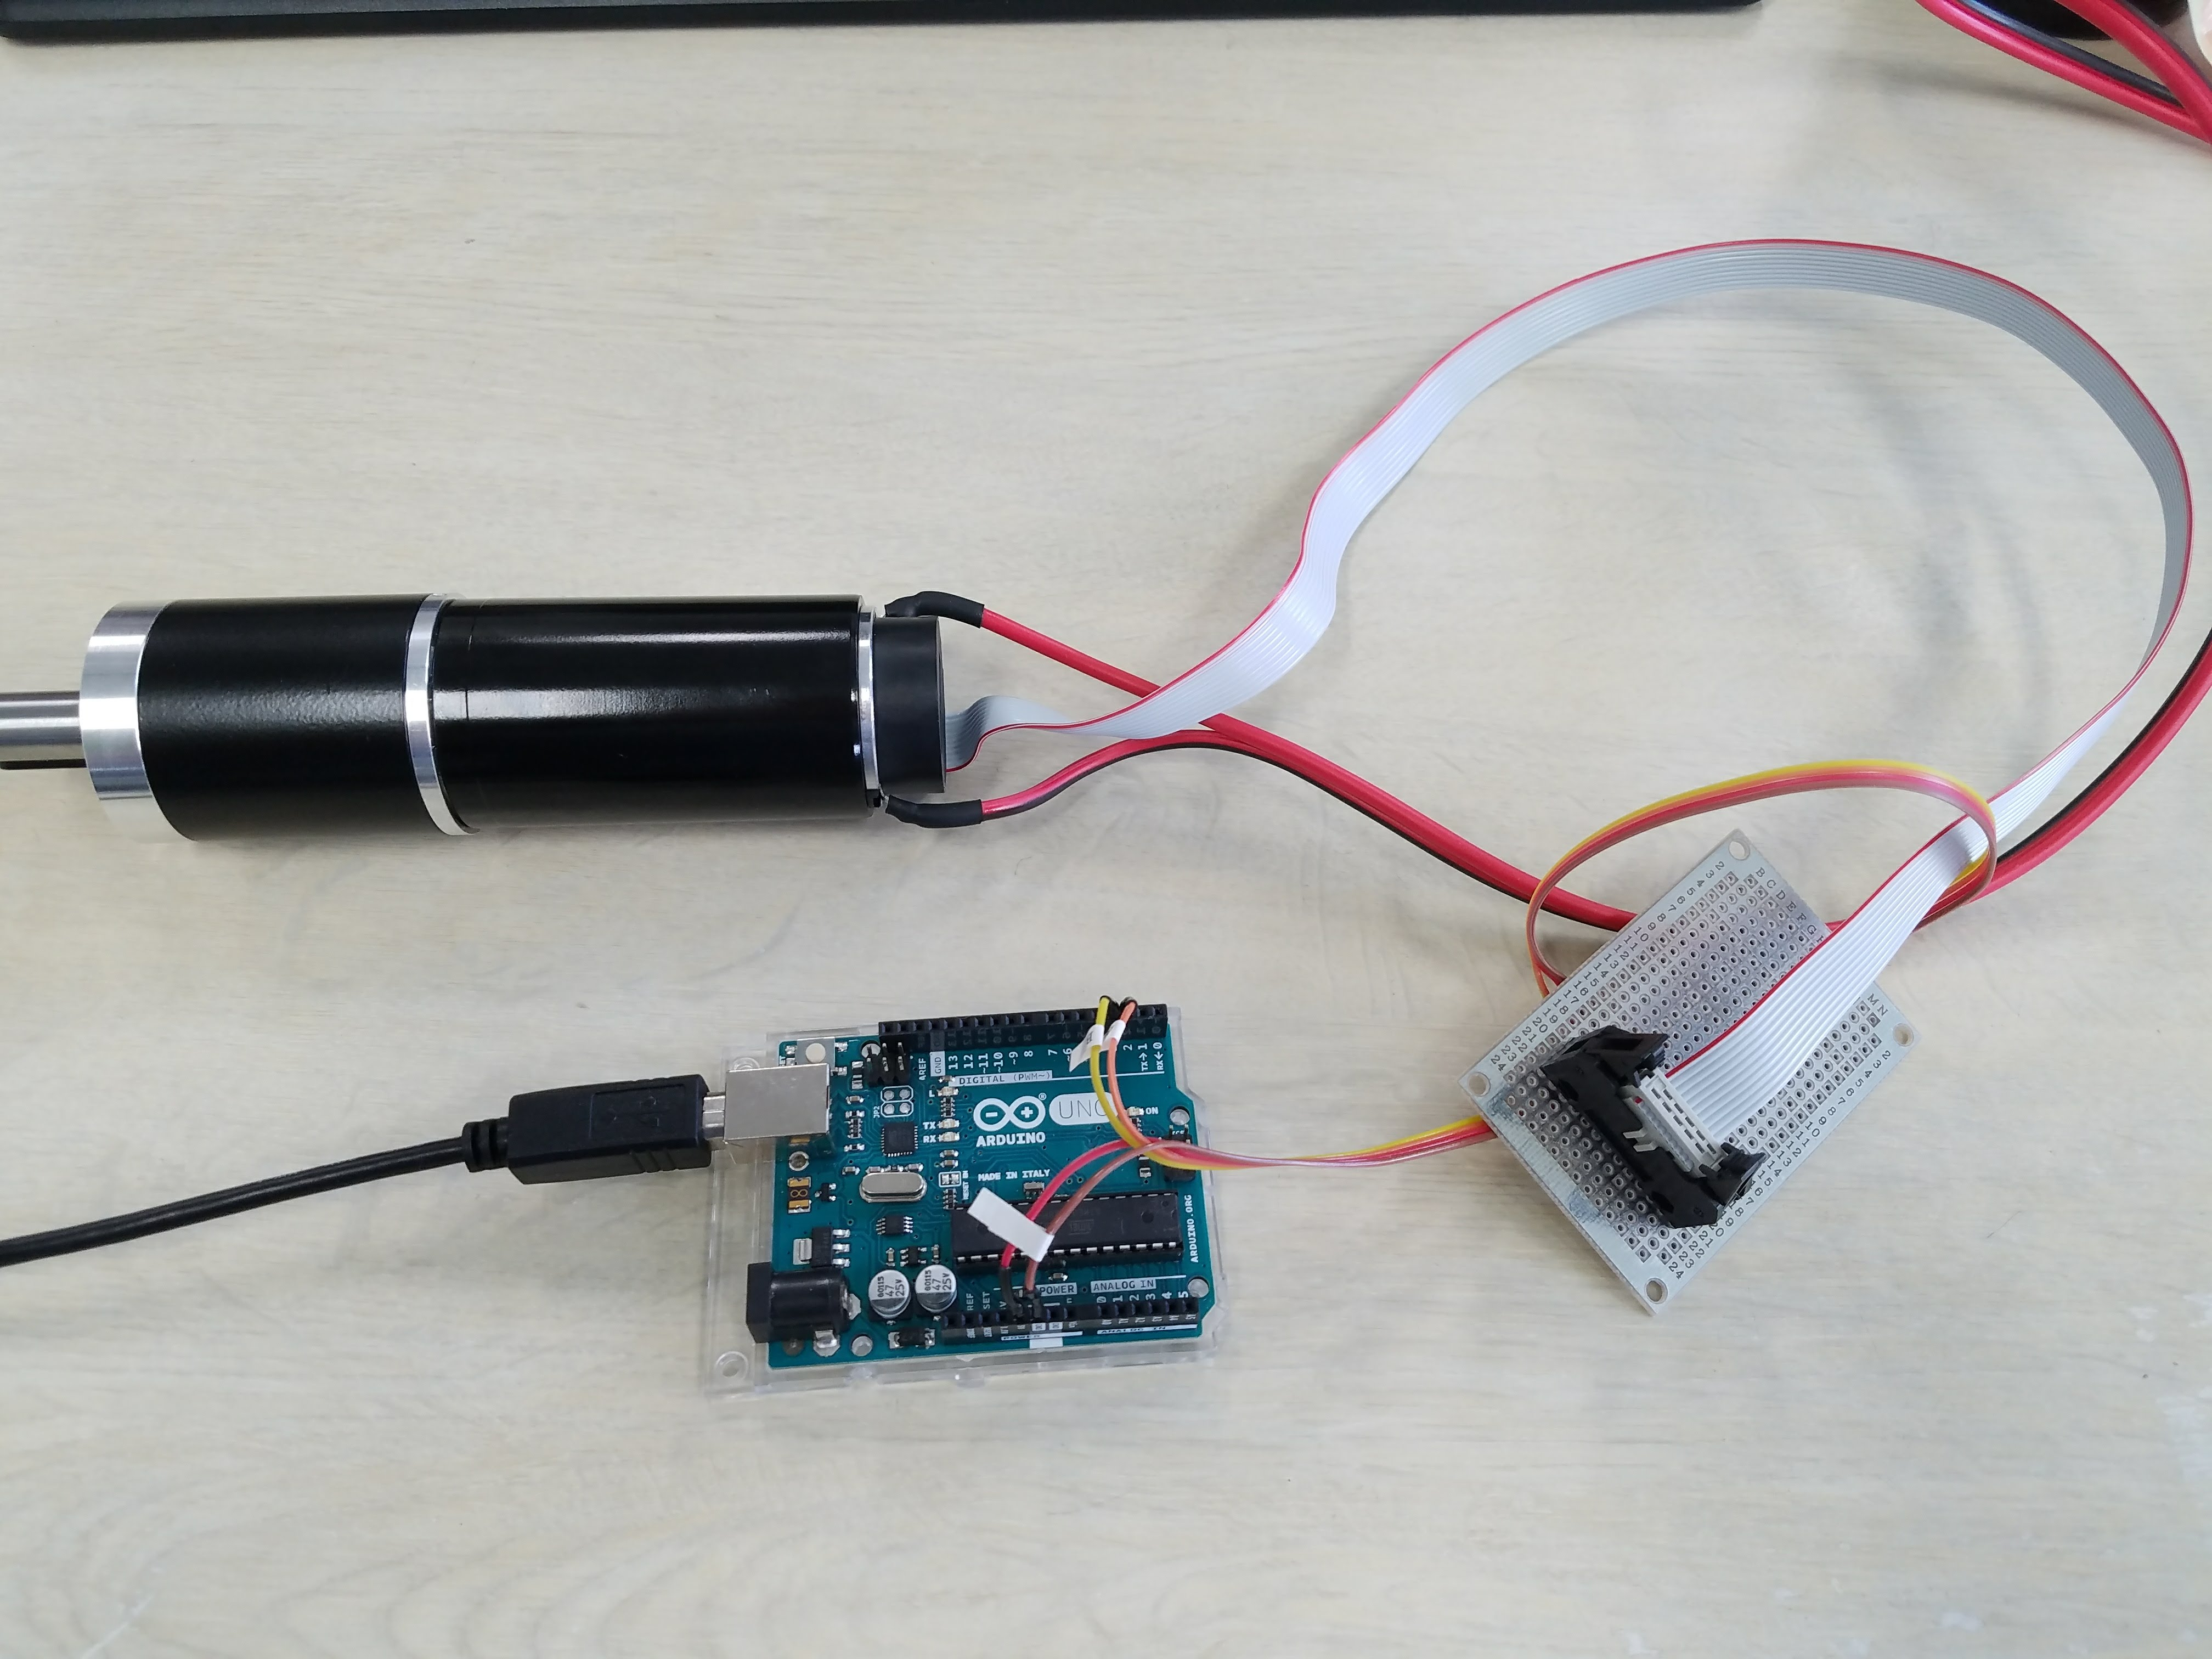
\includegraphics[width=7.0cm,bb=0 0 4032 3024]{cable.jpg}
        \caption{配線全体図}
        \label{ラベル1}
     \end{center}
\end{figure}

\begin{figure}[htbp]
	\begin{center}
      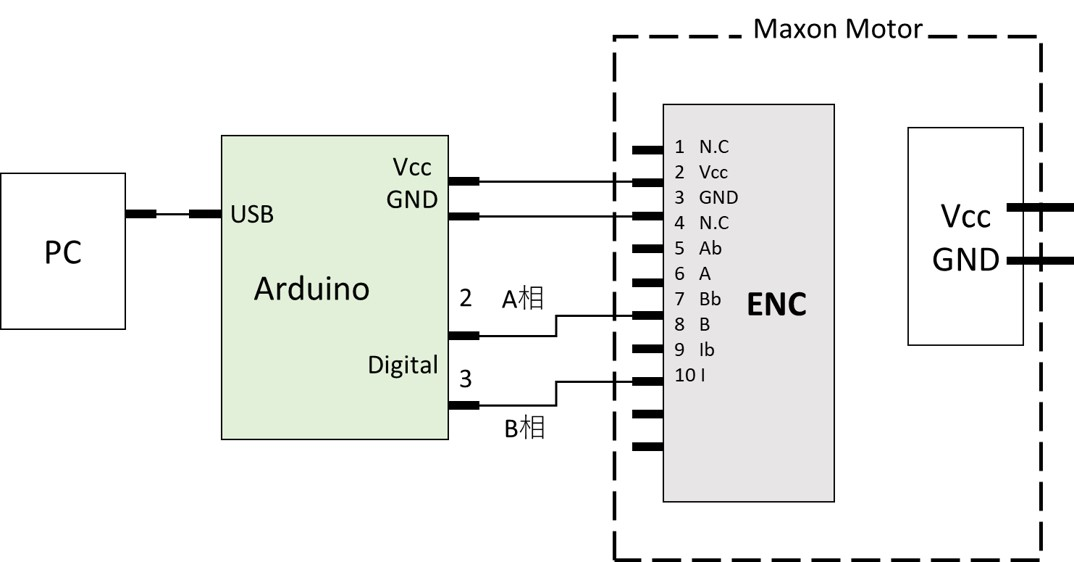
\includegraphics[width=10cm,bb=0 0 1074 562 ]{connect.jpg}
        \caption{maxon motorとArduinoの接続}
        \label{ラベル2}
     \end{center}
\end{figure}

\begin{figure}[htbp]
	\begin{center}
      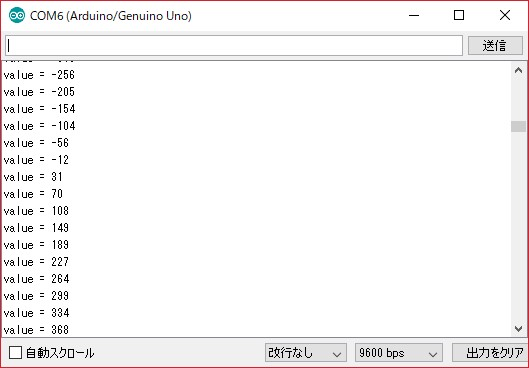
\includegraphics[width=10cm,bb=0 0 529 368]{ex.jpg}
        \caption{実行結果}
        \label{ラベル3}
     \end{center}
\end{figure}





%\subsection{}



%\subsection{}







\section{次の期間の研究}
\begin{itemize}
\item{CAN通信,ROSについて勉強する}
\item{CANalyzerの使い方とロボットの動かし方を学ぶ}
%\item{}
%\item{}
\end{itemize}


%画像の貼り方%
%\begin{figure}[htbp]
%	\begin{center}
%      \includegraphics[width=4.0cm]{.eps}
%        \caption{キャプション}
%        \label{ラベル}
%     \end{center}
%\end{figure}





\end{document}
